\documentclass[12pt,titlepage]{article}


\usepackage{nomencl}
\usepackage[american]{babel}
\usepackage[utf8]{inputenc}
\usepackage[T1]{fontenc}
\usepackage{lmodern}
\usepackage{amsmath,amsfonts,amssymb}
\usepackage{graphicx}
\usepackage{geometry}
\geometry{a4paper}
\usepackage[parfill]{parskip}
\usepackage{graphicx}
\usepackage{amssymb}
\usepackage{epstopdf}
\usepackage{color}
\usepackage[tt]{titlepic}
\usepackage{fancyhdr}
\usepackage{enumerate}
\usepackage{lastpage}
\usepackage{bm}
\usepackage{epstopdf}
\usepackage{listings}
\usepackage{tcolorbox}
\definecolor{codegreen}{rgb}{0,0.6,0}
\definecolor{codegray}{rgb}{0.5,0.5,0.5}
\definecolor{codepurple}{rgb}{0.58,0,0.82}
\definecolor{backcolour}{rgb}{0.95,0.95,0.92}
 
\lstdefinestyle{mystyle}{
    backgroundcolor=\color{backcolour},   
    commentstyle=\color{codegreen},
    keywordstyle=\color{magenta},
    numberstyle=\tiny\color{codegray},
    stringstyle=\color{codepurple},
    basicstyle=\footnotesize,
    breakatwhitespace=false,         
    breaklines=true,                 
    captionpos=b,                    
    keepspaces=true,                 
    numbers=left,                    
    numbersep=5pt,                  
    showspaces=false,                
    showstringspaces=false,
    showtabs=false,                  
    tabsize=2
}
 
\lstset{style=mystyle}

\usepackage[section]{placeins}
\usepackage{amsfonts}
\usepackage{amsmath}
\usepackage{float}
\usepackage{setspace}
\usepackage[justification=centering]{caption}
\usepackage{sidecap}
\usepackage{subcaption}
\usepackage{multirow}
\usepackage[squaren, Gray, cdot]{SIunits}
\graphicspath{{image/}} %chemin par défaut pour aller chercher les images 
\usepackage{url}
\usepackage[utf8]{inputenc}
% FOR DEFINITIONS (https://www.sharelatex.com/learn/Theorems_and_proofs)
\usepackage{amsthm}

\newtheorem{definition}{Definition}[section]
\newtheorem*{definition*}{Definition}
\newtheorem{prop}{Proposition}
\newtheorem*{prop*}{Proposition}
\theoremstyle{remark}
\newtheorem*{remark}{Remark}
\newtheorem*{corollary}{Corollary}
\newtheorem{theorem}{Theorem}[section]
\newtheorem{lemma}[theorem]{Lemma}
\newtheorem*{example}{Example}

% Custom Defines
\usepackage[comma,numbers,sort&compress]{natbib}
\bibliographystyle{plainnat}
\usepackage[pdfstartview=FitH,
            breaklinks=true,
            bookmarksopen=true,
            bookmarksnumbered=true,
            colorlinks=true,
            linkcolor=black,
            citecolor=black
            ]{hyperref}
\newcommand{\rmd}{\textrm{d}}
\newcommand{\norm}[1]{\left\lVert#1\right\rVert}
\newcommand{\bi}[1]{{\ensuremath{\boldsymbol{#1}}}}
\definecolor{gray}{rgb}{0.5,0.5,0.5}

\topmargin=-0.45in      %
%\evensidemargin=0in     %
\oddsidemargin=-0.1in      %
\textwidth=6.8in        %
\textheight=9.2in       %
%\headsep=0.25in         %
\headheight=30.9pt

\begin{document}

% ========== TITLE PAGE ===================================================

\begin{titlepage}
\newcommand{\HRule}{\rule{\linewidth}{1mm}} % Defines a new command for the horizontal lines, change thickness here

\center % Center everything on the page
\includegraphics[width=8cm]{Figs/Cover/polimi.png}\\[1.5cm]
\includegraphics[width=8cm]{Figs/Cover/EPFL.jpg}\\[1.5cm]
%	HEADING SECTIONS
\textsc{\LARGE Master Thesis in Computational Science and Engineering}\\[1.cm]

%	TITLE SECTION
\HRule \\[0.4cm]
{ \huge \bfseries About the convergence of the Graph Laplacian on a 2-sphere}\\[0.4cm] 
\HRule \\[1.5cm]     

%	AUTHOR SECTION
\begin{minipage}{0.4\textwidth}
\begin{flushleft} \large
\emph{}\\
Martino \textsc{Milani}\\
\end{flushleft}
\end{minipage}
~
%	DATE SECTION
{\large \today }\\[2cm] % Date, change the \today to a set date if you want to be precise
\vfill % Fill the rest of the page with whitespace
\end{titlepage}
%\onehalfspacing

% ========== HEADER =======================================================
\pagestyle{headings} \pagenumbering{arabic} \setcounter{page}{1}
\addtolength{\headheight}{\baselineskip}
\lhead{\textbf{Martino Milani}}
\chead{Master Thesis}
\renewcommand{\headrulewidth}{0.4pt}


\begin{abstract}

A fundamental problem in signal processing is to design computationally efficient algorithms to filter signals. In many applications, the signals to filter lie on a sphere. Meaningful examples of data of this kind are weather data on the Earth, or images of the sky. It is then important to design filtering algorithms that are computationally efficient and capable of exploiting the rotational symmetry of the problem. In these applications, given a continuous signal $f: \mathcal S_2 \rightarrow \mathbb R$ on a 2-sphere $\mathcal S_2 \subset  \mathbb R^3$, we can only know the vector of its sampled values $\mathbf f \in \mathbb R^N:\quad (\mathbf f)_i = f(\mathbf x_i)$  in a finite set of points $\mathcal P \subset \mathcal S_2,\quad \mathcal P = \{\mathbf x_i\}_{I=0}^{N-1}$ where our sensors are located. Deferrard et al. in [1] construct a sparse graph $G$ on the vertex set $\mathcal P$ and then use a polynomial of the corresponding graph Laplacian matrix $\mathbf L  \in \mathbb R^{N\times N} $ to perform a computationally efficient - $\mathcal O (N)$ - filtering of the sampled signal $\mathbf f$. In order to study how well this algorithm respects the symmetry of the problem - i.e it is equivariant to the rotation group SO(3) - it is important to guarantee that the spectrum of $\mathbf L$  and spectrum of the Laplace-Beltrami operator $\triangle_\mathcal M$ are somewhat "close".

We study the spectral properties of such graph Laplacian matrix in the special case of [1] where the sampling $\mathcal P$ is the so called HEALPix sampling (acronym for \textbf Hierarchical \textbf Equal \textbf Area iso\textbf Latitude \textbf {Pix}elization) and we show a way to build a graph $G'$ such that the corresponding graph Laplacian matrix $\mathbf L'$ shows better spectral properties than the one presented in [1].

We then started investigating what happens with different samplings of the sphere, less homogeneous than HEALPix and very used in applications. We saw that the graph Laplacian on such samplings perform way worse than on HEALPix. We then investigated other different methods of building the matrix $\mathbf L$. In particular, we studied the Finite Element Method approximation of the Laplace-Beltrami operator on a manifold. The FEM approach do not rely on a point cloud, but on a mesh. Thanks to this it is able to better capture the structure of the manifold even when the sampling is very far from being homogeneous. We compare the FEM and the graph Laplacians on the HEALPix and on the equiangular sampling on the sphere and we show that on HEALPix the graph performs better, on the equiangular sampling it is the FEM that performs much, much better. The FEM approach provides a \textbf{continuous} approximation of the operator whose "quality" depends only on the geometrical properties of the underlying mesh; this means that by knowing a priori the manifold (the sphere in our case) we can build a mesh that is really accurate, leading to a really accurate approximation of the Laplace Beltrami operator that we can then use somehow on the signal sampled anywhere else on the manifold (\textbf{TO UNDERSTAND}). Big question is: how can we filter a signal with the FEM approximation of the Laplace Beltrami? Indeed, its construction is very different from the graph one. A naive alternative would be to use the matrix $B^{-1}L$, that would lead to $\mathcal O(n^2)$ computations. An alternative would be to use the "mass lumping" method (TODO TODAY). \textbf{If it works}, it's awesome! \textbf{Second Big question is: how can we insert such FEM filtering in a layer of a CNN? Meaning, how can we define the back propagation algorithm on $Lx = Bx$?}



\end{abstract}
\pagebreak

\tableofcontents
\pagebreak

%\listoffigures
%\listoftables
%\pagebreak


%*******************************************************************************
%***********************************    Background   *****************************
%*******************************************************************************
%!TEX root = 0.main.tex

\setcounter{page}{1}



%********************************** %First Section  **************************************
\section {Introduction and general background} 

\subsection{Introduction}

Neural Networks (NNs) are popular algorithms for regression and classification tasks. Taking as example classification tasks of mapping the image $I$ into its correct label $C_I$, neural networks perform multiple combinations of linear and non-linear transformations of the image $I$ to assign it a label in $\mathcal C$.  The first \textit{layer} of a neural network transforms the input image $I$ in a vector $\mathbf f_1$ through a function $\phi_1$. $\mathbf f_1$ is used as input of the following layer that transforms it in a second vector $\mathbf f_2$ through a second function $\phi_2$, and so on, until the original image $I$ is mapped into a label $C_I$ by the last, $n$-th layer of the neural network:
$$C_I = \phi_n \circ \phi_{n-1}\circ ... \phi_2\circ\phi_1 (I)$$
 Given a large \textit{training set} of labeled images, a neural network is capable of learning the optimal transformations $\phi_i$ that let it map the input image to its correct label. Since the functions $\phi_i$ have many degrees of freedom - even millions - a neural network is able to learn very complex transformations. This characteristic makes NNs the optimal tool for complex tasks such as image classification, image segmentation, speech recognition and natural language processing.\\

Convolutional Neural Networks (CNNs) are a specific class of neural networks whose layer structure has been specifically designed for image recognition and segmentation. For this purpose, they don't have all the degrees of freedom of a normal, \textit{fully connected} neural network described above: each layer of a CNN has been constrained to only learn transformations of the input that are \textit{invariant} to translation of the input. This means that if used in an image classification task, a translation of the input image will not result in a change of class. The function $\phi_i$ of a CNN are \textit{convolutions} with some kernel that was learned during the training phase. Thanks to their design, training of CNNs is faster - thanks to the smaller number of parameters to be learned compared to a fully connected NN -, it is easier -since there's no need of artificially \textit{augmenting} the dataset with translated copies of the same image -, and leads to very accurate results.\\

Spherical convolutional neural networks (SCNNs) are NNs that have been specifically designed to deal with spherical data, whose layer design makes them \textit{equivariant to rotations of the input}.  Examples of tasks where data is naturally represented on a sphere are (i) climate science, where data is sampled on the surface of the Earth, (ii) cosmology, where observations are naturally projected on a sphere centered around the observer (see Figure \ref{fig:cosmicradiation}), and (iii) virtual reality, where the images are represented on a sphere centered around the player. Being able to come up with designs that are equivariant to rotations brings with it all the advantages that traditional CNNs have brought for traditional (euclidean) image classification tasks: training is faster, easier and results are very accurate. The transformations $\phi_i$ that each layer of a SCNN performs is a \textit{spherical convolution} of the input vector with a kernel learned during the training phase. 

\begin{figure}
	\centering
	\caption{\label{fig:cosmicradiation} Cosmic microwave background map, the oldest electromagnetic radiation in the universe. Source: Wikipedia}
	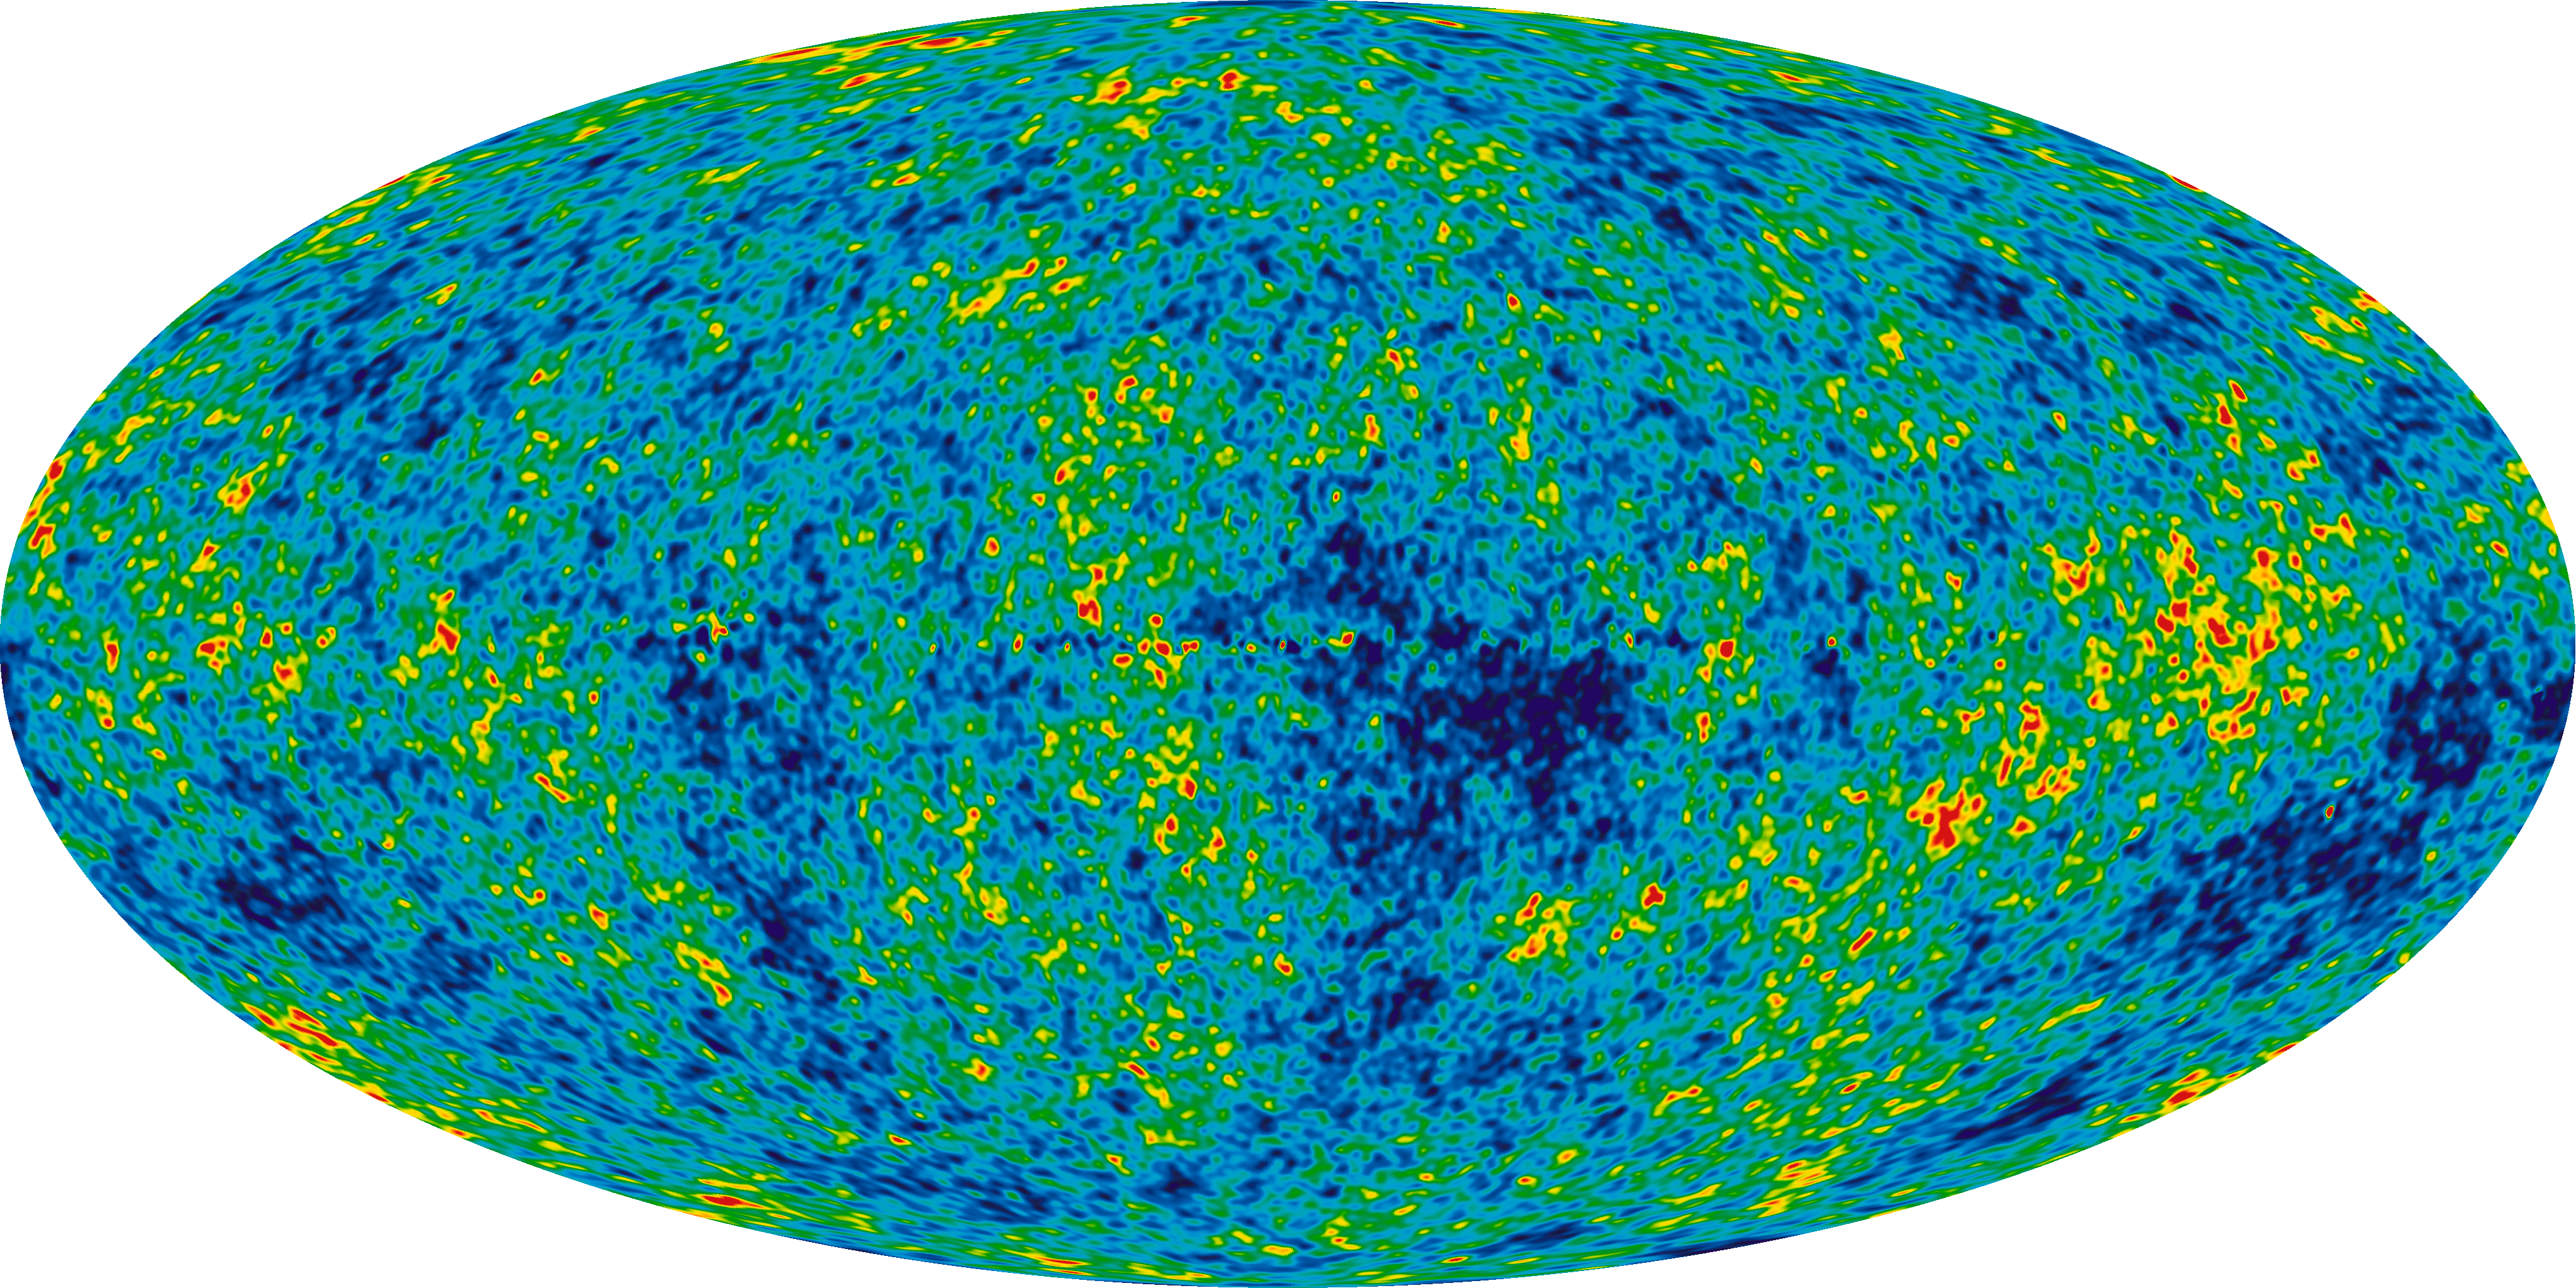
\includegraphics[width=0.4\textwidth]{figs/literaturereview/WMAP.png}
\end{figure}
One of the main issues with traditional SCNNs is the computational complexity of computing at each layer the Spherical Harmonic Transform (SHT) of the data to perform the convolution in the spectral domain. Perraudin et al. \cite{DeepSphere} proposed a Graph Convolutional Neural Network (GCNN) that is almost equivariant to rotations, replacing the SHT with a more efficient Graph Convolution.

In Chapter 1 we start by presenting fundamental concepts of spectral theory on the sphere and we present classical ways of building rotation equivariant neural networks through the use of the SHT.  We present then some basics of Graph Spectral Theory useful to introduce the work of Perraudin et al. DeepSphere \cite{DeepSphere}. We present then a well suited way to build a graph to approximate the Laplace-Beltrami operator on a manifold, the Heat Kernel Graph Laplacian (HKGL) together with some convergence results. In Chapter 2 we study the spectral properties of the graph Laplacian matrix $\mathbf L$ used by Perraudin et al. and we show a way to build a graph $G'$ such that the corresponding graph Laplacian matrix $\mathbf L'$ shows better spectral properties. In Chapter 3 we investigate other different methods of building the matrix $\mathbf L$ better suited to non uniform sampling measures. In particular, we study the Finite Element Method approximation of the Laplace-Beltrami operator on the sphere. We compare the FEM and the graph Laplacian on different samplings of the sphere. We finish by discussing the general problem of how to incorporate geometrical informations about the sphere in the graph, a purely topological object.

\subsection{Fourier Transforms and Convolutions on the 2-Sphere}
[Review of \textit{Computing Fourier Transforms and Convolutions on the 2-Sphere}]
\subsection{Spherical Convolutional Neural Networks}
[Review of \textit{Spherical CNNs}]
\subsection{Graph Spectral Theory} \label{sec:Chapter1: Spectral Graph Theory}
[Review of \textit{The emerging field of Graph Signal Processing}]
\subsection{Deep Sphere V1.0}
[Review of \textit{Deep Sphere}]
\subsection{Belkin's trinity}
[Review of \textit{the Belkin's trinity}]

\subsubsection{Towards a theoretical foundation of Laplacian-based manifold methods}

\subsubsection{Consistency of Spectral Clustering}

\subsubsection{Convergence of Laplacian Eigenmaps}

\pagebreak

%*******************************************************************************
%*********************************** Second Chapter *****************************
%*******************************************************************************
%!TEX root = 0.main.tex
\section{First Month}
\subsection{Daniel Spielman's notes, Jupyter Notebook "Experience1" and meeting of Tuesday 26 February}

One interesting thing:

\begin{theorem}{\textit{Lemma 5.2.1 of Daniel Spielman's Lecture Notes of the course of Spectral Graph Theory (2015)}}
	\label{theo:eigenvectors on the ring}
	The Laplacian of the 2-Nearest-Neighbours ring graph $R_n$ on $n$ equispaced vertices has eigenvectors
	$$\mathbf x_k(u) = \cos(2k\pi u/n)$$
	$$\mathbf y_k(u) = \sin(2k\pi u/n)$$
	for $0\leq k\leq n/2$, ignoring $\mathbf y_0 = \mathbf 0$ and for even $n$ ignoring $\mathbf y_{n/2}$ for the same reason. Eigenvectors $\mathbf x_k, \mathbf y_k$ have eigenvalues $2-2\cos(2\pi k/n)$
\end{theorem}

This lemma make us realize the fact that for a Graph Laplacian it is possible to have eigenvectors equal to the spherical harmonics sampled in the nodes, but has completely different eigenvalues! Furthermore, if I artificially build a matrix $L'=U\Lambda'U^T$ such that $L=U\Lambda U^T$ but with $\Lambda'=\text{diag}\{-1, -4, -4, -9, -9, ...\}$ the eigenvalues of the operator  
$$\triangle \Phi(\rho, \theta) = \frac{1}{\rho}\partial_\rho \left(\frac{1}{\rho}\partial_\rho \Phi\right) + \frac{1}{\rho^2}\partial_{\theta\theta}\Phi$$ 
Laplace-Beltrami on the circle  So, this tells us that the problem proposed by Micha\"el
\begin{equation}\label{eq:michaelsproblem}
	W^\star = \arg\min_W||U-\hat U||, \quad L=D-W,\quad LU=U\Lambda
	 \hat U = \text{"Spherical harmonics sampled in the point set P"}
\end{equation}

could be badly posed, in the sens that once found the weights $W^\star$ that give us the $U^\star$ realizing the minimum above, we have no clue of which eigenvalues to set in order to retrieve a true Graph Laplacian (positive diagonal, negative entries, symmetric, row/column sum equal to $0$).\\
Nathana\"el proposes a different approach. After having observed that given a non-uniform sampling (that's the setting we are aiming at) the vectors of the spherical harmonics sampled in the point set $P$ won't be orthogonal, and thus a spectral decomposition of the Laplacian will never realize Micha\"el's problem \ref{eq:michaelsproblem} he proposes the following problem:
\begin{equation}\label{eq:nathanaelsproblem}
	\arg\min_W||L\hat U-\hat U\hat \Lambda||_\mathcal F,\quad L=D-W,\quad  W>0,\quad D=\text{diag}\{\sum_{i}(W)_{i,j}\}
\end{equation}

where $\hat{\Lambda}, \hat{U}$ are respectively the eigenvalues and eigenvectors of $\triangle_\mathcal M$ the operator of Laplace-Beltrami sampled in the point set P. In this way we get the graph laplacian that has the closest spectral decomposition to the "true" one. The problem \ref{eq:nathanaelsproblem} can be rewritten in the following form 

\begin{equation}\label{eq:nathanaelsproblem2}
[w^\star\ \lambda^\star]^T = \arg\min_W||A[w\ \lambda]^T||_2^2
\end{equation}

However, Micha\"el is not convinced by the fact that the form of the problem seems redundant: $\lambda=\lambda(w)$ is a function of $w$. So, the optimization is done on both $\lambda, w$ that can't respect the relationship $\lambda=\lambda(w)$. At the end only one of the two arguments of the minimization problem $[w^\star\ \lambda^\star]^T$ will be used to obtain the second according to the relation $\lambda=\lambda(w)$.

Waiting for Nathan\"el's notes to make this passage clearer


\subsection{Nath's problem}

Given a matrix $U$, we would like to find a valid graph such that
its eigenbase is as close to $U$ as possible. Note that $U$ might
contain only a few eigenvectors (be rectangular) and might not be
orthogonal, i.e.: $UU^{*}\neq I$.

\subsection*{Some remarks}
\begin{itemize}
	\item The Fourier basis (DFT) is probably only available for a circulant
	matrix
	\item If $U$ is not orthogonal, it is useless to try to use it directly
	to build the Laplacian
	\item The value of the eigenvalues $\Lambda$ cannot be known in advance
	\item Learning a graph given an eigenbasis has been done \cite{pasdeloup2018characterization,shafipour2017network}
	It does not work well according to me and I do not like the papers.
	\item For graph learning, the best paper to read is probably \cite{kalofolias2016learn}.
	Some more advanced results are availlable in \cite{kalofolias2018large}.
	I might be biased in recommending these two papers. You can check
	the references inside if you want to see more.
\end{itemize}

\subsection*{Problem formulation}

Solving the problem directly, i.e. searching for $U$ and $\Lambda$
is, according to me, too complicated. Hence I propose an indirect
solution. Instead of searching for $U,\Lambda$ such that $L=U\Lambda U^{*}$,
we search for $L$ such that:

\[
LU=\Lambda U
\]
We formulate the optimization problem as:

\[
\text{arg}\min_{w}\|LU-\Lambda U\|_{F}^{2}\hspace{1em}\text{s.t.}\lambda^{*}\mathbf{1}=1,w\geq0,\lambda\ge0
\]
Here $w\geq0,\lambda\geq0$ ensure that we have a valid graph and
$\lambda^{*}\mathbf{1}=1$ ensures that the trivial solution $w=0$
is not selected. Now $L$ is linearly linked to $W$ by
\[
L_{ij}=\begin{cases}
-W_{ij} & \text{if }i\ne j\\
\sum_{i}W_{ij} & \text{otherwise.}
\end{cases}
\]
Let us write this operator 
\[
\ell=O_{L}w=\text{vec}\left(\text{diag}(\text{mat}(w)\mathbf{1})-\text{mat}(w)\right)
\]
For simplicity, we assume $W_{i,i}=0$. Furthermore $LU$ is also
a linear operation. Let us write the operator $O_{U}.$ We have 
\begin{align*}
\left(LU\right)_{o,p} & =\sum_{j}L_{o,j}U_{j,p}\\
& =U_{o,p}\sum_{i}W_{io}-\sum_{j}W_{o,j}U_{j,p}
\end{align*}
Similarly, we have we define $O_{\Lambda}$ such that 
\[
O_{\Lambda}\lambda=\text{vec}(\text{diag}(\lambda)U).
\]
Eventually, we have 
\[
\|LU-\Lambda U\|_{F}^{2}=\left\Vert A\left[\begin{array}{c}
w\\
\lambda
\end{array}\right]\right\Vert _{2}^{2}
\]
where $A=\left[\begin{array}{cc}
O_{U}O_{L} & O_{\Lambda}\end{array}\right]$. The problem can be solved with a quadratic programing (QP) solver.

\subsection*{Alternative problem formulation}

The previous problem formulation penalizes mostly the spectral modes associated with high eigenvalues. In an attempt to solve this issue, we can formate the quadratic term as

\[
\|\Lambda^{-1}LU-U\|_{F}^{2}=\|\Lambda^{-1}(D-W)U-U\|_{F}^{2}.
\]
This implies that the variables $w,\lambda$ are mixed and the problem
is no longer convex. Let $T=\Lambda^{-1}(D-W)=\Lambda^{-1}D-\Lambda^{-1}W,$
then 
\[
T_{ij}=\begin{cases}
-\lambda_{i}^{-1}W_{i,j} & \text{if }i\ne j\\
\lambda_{i}^{-1}\sum_{j}W_{i,j} & \text{otherwise.}
\end{cases}
\]
Now if we were to minimize the quadratic $\|TU-U\|_{F}^{2}$, a trivial
solution would be $T=I.$ I do not think, this leads anywhere. 

\subsection*{Other ideas}

Which is the closest $U$ from $U_{G}$ such that it remains orthonormal?
\[
\text{arg}\min_{U}\|U_{G}-U\|_{F}\hspace{1em}UU^{*}=I
\]

\subsection{Weeks 2-3 (26 Feb - 12 Mar)}

\subsubsection*{Nath's problem $\mathbf{\arg \min ||LU-U\Lambda||}$}
I implemented Nathana\"el's problem in the file 04\_optimization.py on a sampled ring, in order to have the possibility to refer to theorem \ref{theo:eigenvectors on the ring} that I correctly implemented in the notebook 02\_Experience1.py. Theorem \ref{theo:eigenvectors on the ring} tells us that in some cases (uniform sampling) it is possible to have as G-eigenvectors the sampled $\mathcal{M}$-eigenvectors, but with different eigenvalues! This means (as we understood with Micha\"el on Tuesday 12 March) that if we want to engineer a graph filter $F_G(f_{(P)}) = Uh(\Lambda_G)U^Tf_{(P)}$ such that is acts on the graph-spectrum of the sampled signal $f(P)$ as the continuous $\mathcal{M}$-filter $F_\mathcal M(f)_{(x)} =  \mathcal F^{-1}\left(\sum_i h_{\mathcal M}(\lambda_{\mathcal M, i}) Y_i(\omega)\right)(x)$ acts on the $\mathcal M$-spectrum of the continuous signal $f(x)$ we need to \textit{identify the graph eigenvalues with the corresponding $\mathcal M$-eigenvalues to make sure that $h_G(\lambda_{i,G}) = h_{\mathcal M}(\lambda_{i,\mathcal M}) $}.\\
We observed that the result of the optimization for uniform sampling and for non-uniform sampling. Results are the in PDM/codes/04\_optimization/04\_figs. We see a good correspondence between $\Lambda^\star$ and the eigenvalues of the optimal Laplacian $L^\star$. However, we do not observe a good correspondence between the eigenvectors and the sampled spherical harmonics. However, it is really hard to interpret the scalar product between the vectors of the sampled spherical harmonics and the eigenvectors when the sampling is not uniform!\\
\textbf{TO DO}: to compare the graph eigenvectors with the sampled spherical harmonics we did a scalar product of the vectors. However, we need to do a proper NUDFT (Non Uniform Discrete Fourier Transform https://en.wikipedia.org/wiki/Non-uniform\_discrete\_Fourier\_transform), that is a proper discretization of the integral $\int_{\mathcal S_1} u_i(x) Y_j(x) dx$ where $u(x)$ is the continuous graph eigenvector (\textbf{QUESTION}: what does this mean?) and $Y_j$ is the $j$-th spherical harmonic. The scalar product in $\mathbb R^N$ of the sampled signals corresponds to the scalar product in $L_2(\mathcal S_1)$ and thus to a DFT only for band-limited signals and in case of uniform sampling, since the vectors of the sampled harmonics are orthonormal!
\subsubsection*{G-orthogonality and $\mathcal M$-orthogonality}
It is key to distinguish between the concepts of G-orthogonality and $\mathcal M$-orthogonality. This generated a lot of confusion in the past weeks. The question is the following: what is the SHT of a signal? The answer depends on the functional setting of the class of signals we want to work with. If we define the class of signals 

$$\mathcal F = \{f: \mathcal M \rightarrow \mathbb R: SHT(f)_i = 0\quad \forall i \geq N \}$$ 

and the sampling set $P = \{x_i \in \mathcal M\}_{i=0}^N$ we have that 

$$\forall f\in \mathcal F,  \forall x\in \mathcal M \quad \mathbf f(x)=\sum \hat f_i Y_i(x)$$

Where $\mathbf {\hat f} = \{\hat f_i\} = SHT(f)$. Thus on the sampling point set $P$ we can write

$$\forall f\in \mathcal F\quad \mathbf f_{(P)}=\sum \hat f_i Y_{i(P)} = Y_P \mathbf {\hat  f}$$


If the matrix $Y_P$ of the sampled spherical harmonics is full rank, for these signals it is true that

$$\forall f \in \mathcal F \quad SHT(f) = \mathbf{\hat f} = Y_P^{-1} f_{(P)}$$

However, for a general signal on the manifold, the $SHT(f)$ is given by the Type 2 - Non Uniform Discrete Fourier Transform (Type 2 NUDFT). From my understanding, it provides an approximation of the transform since a non-uniform sampling is capable of catching all the frequencies, but once we cut the Fourier series we do not have a Shannon Theorem (perfect reconstruction of band-limited signals).\\
The NUDFT requires to set as a parameter the maximum frequency we want to project our signal on.

On the sphere the NASA provides us with the function \lstinline {anafast} that implements a Type2-NUDFT on the HEALPix sampling out of the box. This program performs harmonic analysis of the HEALPix maps up to a user specified maximum spherical harmonic order $l_{max}$.

\subsubsection*{The first question}
For a signal $f: \mathcal M \rightarrow \mathbb R$ define $\mathbf{\hat f}_G = U^T f(P)$ and  $\mathbf{\hat f}_\mathcal M = SHT(f)$.
The question is the following: is there a graph Fourier basis $U: U^TU=I$ such that $\mathbf{\hat f}_G = \mathbf{\hat f}_\mathcal M \forall f$?

If this is true, I have a graph such that the G-spectrum is equal to the $\mathcal M$-spectrum. However, nothing is said about the eigenspaces. \textbf{In any case, the answer to this question is NO}. 
In the setting of band limited signals $\mathcal F = \{f: \mathcal M \rightarrow \mathbb R: SHT(f)_i = 0\quad \forall i \geq N \}$  if the matrix $Y_P$ is full rank we have that $U$ has to be equal to $Y$ since $\mathbf{\hat f_G} = U^Tf(P)$ and $\mathbf{\hat f_\mathcal M} = Y_P^{-1}f(P)$. Even if we relax the request asking
 
$$(\mathbf{\hat f}_{G})_i = (\mathbf{\hat f}_{\mathcal M})_i \quad\forall i \leq n<N \quad \forall f$$

still this is impossible since from this it must follow that the first $n$ columns of $Y^{-1}_P$ are orthonormal, not true for a general sampling $P$.


\subsubsection*{The second question}
Is it possible to find a graph such that the G-eigenspaces are aligned with the $\mathcal M$-eigenspaces? \textbf{Problem: It is a badly formulated question! It doesn't mean much if we do not specify it better.} The formulation 

\[Y^TU = 
\left[ {\begin{array}{ccccc}
	B_{1\times 1} & 0 & 0 & 0 & ...\\
	0 & B_{3\times 3} & 0 & 0 & ...\\
	0 & 0 & B_{5\times 5} & 0 & ...\\
	0 & 0 & 0 & B_{7\times 7} & ...\\
	... & ... & ... & ... & ...\\
	\end{array} } \right]
\]

is not clear since we are projecting the graph eigenvectors on the sampled spherical harmonics in $\mathbb R^N$, but this corresponds to nothing!! What we want is a concept of "alignment" in the continuous domain: so, a better formulation could be the following:


\[SHT(U) = 
\left[ {\begin{array}{ccccc}
	B_{1\times 1} & 0 & 0 & 0 & ...\\
	0 & B_{3\times 3} & 0 & 0 & ...\\
	0 & 0 & B_{5\times 5} & 0 & ...\\
	0 & 0 & 0 & B_{7\times 7} & ...\\
	... & ... & ... & ... & ...\\
	\end{array} } \right]
\]

But again here we have a problem: when we write $SHT(U)$ we are imagining the eigenvectors $\mathbf u_i\in \mathbb R^N$ as traces of a continuous signal $u_i(x): \mathcal M \rightarrow \mathbb R$ and what we want is actually the $SHT(u_i(x))$. The problem is that on a uniform sampling we are limited by the Shannon theorem, that means we can reconstruct the spectrum of $u_i(x)$ only up to a certain frequency, and on a non-uniform sampling we do not know anything at all! On a non-uniform sampled signal there's no way of reconstructing the spectrum, we can only approximate it with a NUDFT. 
\paragraph{Let's now limit ourself to the usual class of band-limited signals.} We know that

$$f(x) = \sum_{i=0}^N \alpha_i Y_i(x)$$

If we suppose that the graph eigenvectors $\mathbf u_j \in \mathbb R^N$ are the trace on the vertices of a "continuous graph eigenvector" $u_j(x) \in \mathcal F$ then we know that 

$$u_j(x) = \sum_{i=0}^N \alpha^j_i Y_i(x)$$

and 

$$SHT(u_i) = Y_P^{-1}u_j(P) = Y_P^{-1}\mathbf u_j$$

so the question becomes
\begin{equation}
SHT(U) = Y_P^{-1}U = \begin{bmatrix}
		B_{1\times 1} & 0 & 0 & 0 & ...\\
		0 & B_{3\times 3} & 0 & 0 & ...\\
		0 & 0 & B_{5\times 5} & 0 & ...\\
		0 & 0 & 0 & B_{7\times 7} & ...\\
		... & ... & ... & ... & ...
		\end{bmatrix} \label{eq:SHT(U)}
\end{equation}


A procedure of proving that this is impossible by absurd could be the following: multiplying eq \ref{eq:SHT(U)} by $Y_P$ we have that

$$
U = Y_P\begin{bmatrix}
B_{1\times 1} & 0 & 0 & 0 & ...\\
0 & B_{3\times 3} & 0 & 0 & ...\\
0 & 0 & B_{5\times 5} & 0 & ...\\
0 & 0 & 0 & B_{7\times 7} & ...\\
... & ... & ... & ... & ...
\end{bmatrix}
$$
 that rewritten column by columns becomes:

 $u_0 = \alpha_1\mathbf Y_0$\\
 $u_1 = \alpha_1^1 \mathbf Y_1 + \alpha_2^1 \mathbf Y_2+ \alpha_3^1 \mathbf Y_3$\\
 $u_2 = \alpha_1^2 \mathbf Y_1 + \alpha_2^2 \mathbf Y_2+ \alpha_3^2 \mathbf Y_3$\\
 $u_3 = \alpha_1^3 \mathbf Y_1 + \alpha_2^3 \mathbf Y_2+ \alpha_3^3 \mathbf Y_3$\\
 ...\\
 
 and so on. I think that the answer to this question is again a no-no: since we must impose $UU^T=I$, this means that we have to find an orthogonal basis of each eigenspace 
 $\text{span}\{\mathbf Y_0\} = \text{span}\{\mathbf u_0\},  \text{span}\{\mathbf Y_1, \mathbf Y_2, \mathbf Y_3\} = \text{span}\{\mathbf u_1, \mathbf u_2, \mathbf u_3\}, \text{span}\{\mathbf Y_4, \mathbf Y_5, \mathbf Y_6, \mathbf Y_7, \mathbf Y_8\}=\text{span}\{\mathbf u_4, \mathbf u_5, \mathbf u_6, \mathbf u_7, \mathbf u_8\}$, etc. etc. (no problem) but the problem comes in when we must impose the $\mathbb R^N$-orthogonality between the different basis of the eigenspaces! This cannot be assured in general. \textbf{TO DO: if you're not convinced by the impossibility of this, find a counter example just with the first two eigenspaces ($|P|=4 \implies \mathbf u_i, \mathbf Y_i \in \mathbb R^4, i=0,1,2,3$)}

\pagebreak

%!TEX root = 0.main.tex

\section{The Belkin's trinity}
\subsection{Towards a theoretical foundation of Laplacian-based manifold methods}

In this paper they present two results: a pointwise probabilistic convergence of \textbf{the extension of the graph Laplacian} 
\begin{definition}{Graph Laplacian}
	$$ \left(\mathbf L_n^t\right)_{ij}=\begin{cases}
	-w_{ij}, & i\neq j\\
	\sum_{k}w_{ik}, & i=j
	\end{cases}$$
\end{definition}
\begin{definition}{Point cloud Laplace operator}
	$$L_n^t:\quad(L_n^tf)(y) = \frac{1}{n}f(y)\sum_i e^\frac{||x_i-y||}{4t}-\frac{1}{n}\sum_ie^\frac{||x_i-y||}{4t}f(x_i)$$
\end{definition}
\begin{definition}{Functional approximation to the Laplace-Beltrami operator} \label{eq:L^t}
	$$L^tf(p) :=  \frac{1}{ (4\pi t)^{\frac{k+2}{2}}} \int_\mathcal Me^{-\frac{||p-x||^2}{4t}}\left(f(x)-f(p)\right)d\mu(x)$$
\end{definition}

\begin{theorem}{Pointwise convergence}
	$$\forall f \in C^\infty(\mathcal M)\quad  C\frac{(4\pi t_n)^{-\frac{k+2}{2}}}{n} L_n^t f(\bf x) \xrightarrow{n\to\infty}\triangle_\mathcal M f(\bf x)$$
\end{theorem}


and a uniform (pointwise convergence of the operator) one
\begin{theorem}{uniform convergence}
	$$\sup_{x\in\mathcal M, f\in \mathcal F_C}\left| C\frac{(4\pi t_n)^{-\frac{k+2}{2}}}{n} L_n^t f(\bf x) - \triangle_\mathcal M f(\bf x) \right|\xrightarrow{n\to\infty}0
	, \quad \mathcal F_C = \left\{f\in C^\infty(\mathcal M), f^{(i)}(x)\leq M, i=1,2,3\right\}$$
\end{theorem}


here nothing is said about convergence of the spectra, plus there's nothing written about the relationship between $\mathbf{Eig} L_n^t$ (the eigenfunctions and eigenvalues of the extension of the graph Laplacian) and $\mathbf {Eig} \mathbf {L}_n^t$ (the eigenvectors and eigenvalues of the matrix Laplacian).

Theorem 1 is proven by simple analysis arguments and by Hoeffding's formula (probability). 
First, by the simple law of large numbers, we have that for a fixed $t>0$, a fixed function $f$ and a fixed point $p\in\mathcal M$
\begin{equation}\label{eq:pointwise convergence of laplacian discrete approximation}
\lim_{n\to\infty}\frac{1}{tn}\frac{1}{ (4\pi t)^{\frac{k}{2}}}L_n^tf(p)= L^tf(p)
\end{equation}




To prove the convergence of $L^t$ to $\triangle_\mathcal M$, then we need three steps, that we can recycle completely. They use the fact that thanks to the exponential map the heat kernel centered on $p$ on any manifold can be approximated by a Gaussian in the ambient Euclidean space in a small neighborhood of $p$, and the relationship between Euclidean distances and geodesic distances.

\textbf{In order to adapt this proof to our needs, we just need to find an alternative to the law of large numbers (LLN) used to prove \ref{eq:pointwise convergence of laplacian discrete approximation}}

Theorem 2 is proven with arguments of Functional Analysis: Ascoli-Arzelà, compact convergence in Sobolev spaces, etc.etc...

\subsection{Consistency of Spectral Clustering}
 $$ \mathbf{Eig} \mathbf{L}^t_n \xrightarrow[a.s.]{n\to\infty} \mathbf{Eig} L^t $$
It aims at proving the convergence of eigenvalues and eigenvectors of random graph Laplacian matrices for growing sample size. They present two results: one for the normalized Laplacian and one for the unnormalized Laplacian. Since the matrix eigenvectors grow in dimension as the sample size increases, standard convergence arguments can not be applied. However, they show that there exists a function $f\in C(\mathcal M)$ such that the difference between the eigenvector $v_n$ and the restriction of $f$ to the sample converges to $0$

$$||v_n-\rho_nf||\rightarrow 0$$

To do so they see the eigenvector $v_n$ as the restriction to the sample of a continuous eigenfunction $f_n$ of some continuous operator $U'_n$ that acts on the space $C(\mathcal M)$. Then they use the fact that 

$$||v_n-\rho_nf||_\infty = ||\rho_nf_n-\rho_nf||_\infty\leq ||f_n-f||_\infty$$


So, it will just be necessary to show that  $$||f_n-f||_\infty\rightarrow 0$$
 \textbf{compact convergence} of both matrices towards $L^t$ (where $\mathcal M$ is a compact metric space) in the Banach space of the continuous functions $(C, ||\cdot||_\infty)$. 

Compact convergence ensures convergence of spectral properties in the following sense: for isolated eigenvalues of the limit operator $\triangle_\mathcal M$ with finite multiplicity we have convergence of eigenvalues and eigenspaces but not convergence of eigenfunctions. for isolated simple eigenvalues of the limit operator we have also convergence of the eigenfunctions!

The proof consists in three steps:
\paragraph{Step 1} Construct a bounded operator $U'_n$ on the Banach space $(C(\mathcal M), ||\cdot||_\infty)$ such that restricted on the sampled values behaves like $\mathbf{L}'_n$. Then, construct an operator $U'$ such that for the law of large numbers for a fixed $f$ and for a fixed $x$, $U'_nf(x) \xrightarrow U'f(x) $
\paragraph{Step 2} Here they establishes the connection between the spectra of $L'_n$ and $U'_n$. In particular, they prove a one-to-one correspondence between the eigenfunctions and eigenvalues of $U'_n$ and the eigenvectors and eigenvalues of $L'_n$, provided that satisfy $\lambda\notin \{1\}=\sigma_{ess}(U'_n)= \sigma_{ess}(U')$.
\paragraph{Step 3} Here we prove compact convergence:

$$U'_n \xrightarrow[n\to\infty]{c,\ a.s.}U'$$

At the light of compact convergence and on the analysis of the essential spectrum of $U'_n, U'$ and the one-to-one correspondence of the spectra done in step 2, given Proposition 6 \textit{Perturbation results for compact convergence} we get to the following result

\begin{theorem}
	Let $\lambda\neq 1 $ be an eigenvalue of $U'$ and $M\subset \mathbb C$ an open neighborhood of $\lambda$ such that $\sigma(U')\cap M=\{\lambda\}$. Then:
\begin{enumerate}
	\item Convergence of eigenvalues: The eigenvalues in$\sigma(L'_n)\cap M$ converge to $\lambda$ in the sense that every sequence $(\lambda_n)_{n\in\mathbb N}$ with $\lambda_n\in\sigma(L'_n)\cap M$ satisfies $\lambda_n\rightarrow \lambda$ almost surely.
	\item Convergence of spectral projections: There exists some $N\in\mathbb N$ such that for $n>N$, the sets $\sigma(U'_n)\cap M$ are isolated in $\sigma(U'_n)$. For $n>N$, let $Pr'_n$ be the spectral projection of $U'_n$ corresponding to $\sigma(U'_n)\cap M$, and $Pr$ the spectral projection of $U$ for $\lambda$. Then $Pr'_n\xrightarrow p Pr a.s.$
	\item Convergence of eigenvectors: if $\lambda$ is a single eigenvalue, then the eigenvectors of $L'_n$ converge a.s. up to a change of sign: if $v_n$ is the eigenvector
	of $L'_n$ with eigenvalue $\lambda_n$, $v_{n,i}$ its i-th coordinate, and $f$ the eigenfunction of eigenvalue $\lambda$, then there exists a sequence $(a_n)_{n\in\mathbb N}$ with $a_i \in \{+1,-1\}$ such that $\sup_{i=1,...,n} |a_nv_{n,i} - f(X_i)| \rightarrow 0$ a.s. In particular, for all $b \in\mathbb R$, the sets $\{a_nf_n > b\}$ and $\{f > b\}$ converge, that is, their symmetric difference satisfies $P(\{f > b\}\triangle\{a_nf_n > b\}) \rightarrow 0$.
\end{enumerate}
\end{theorem}

A similar theorem is stated also for non-normalized Laplacian matrix, although the arguments stay the same.
\subsection{Convergence of Laplacian Eigenmaps}
Here all the pieces are put together. 

 $$ \mathbf{Eig} \mathbf{ L}^t_n \xrightarrow[a.s.]{n\to\infty} \mathbf{Eig} L^t \xrightarrow{t\to0} \mathbf{Eig} \triangle_\mathcal M $$
 
 \begin{theorem}
 	Let $\lambda_{n,i}^t$ be the ith eigenvalue of $\hat L_n^t$ and $e^t_{n,i}$ be the corresponding eigenfunction (which for each fixed i will be shown to exist for t sufficiently small). Let $\lambda_{i}$ be the ith eigenvalue of $\triangle_\mathcal M$ and $e_{i}$ be the corresponding eigenfunction. Then there exists a sequence $t_n\rightarrow 0$ such that
 	
 	$$\lim_{n\rightarrow\infty} \lambda_{n,i}^{t_n}=\lambda_i$$
 	$$\lim_{n\rightarrow\infty}||e_{n,i}^{t_n}(x) - e_i(x)||_2 = 0$$
 	
 	where the limits are in probability.
 	
 \end{theorem}

\paragraph{Step 1: Spectral convergence of the empirical approximation $\mathbf{ L}_n^t$ to $L^t$}
Recycle the work of \textbf{Consistency of Spectral Clustering} with the analysis of the essential spectrum of the limit operator $\sigma_{ess}(L^t)$.
\paragraph{Step 2: Spectral convergence of the functional approximation $L^t$ to $\triangle$}
Really hard. Uniform operator convergence does not hold, however spectral convergence is still assured in theorem 4.1 of the paper. This part, although really hard, will stay the same!


\section{Pointwise convergence in the HEALPix case}

Getting inspired from the work flow presented above, we try to replicate the first theorem obtained in \textbf{Towards a theoretical foundation of Laplacian-based manifold methods} but not in the case of random Laplacians, but in the case of deterministic ones where the sampling is given by the HEALPix scheme. This analysis will be a preparatory work to further studies, since as we pointed out so far, from this kind of convergence nothing is said about the convergence of eigenvalues and eigenvectors. However, this study could maybe tell us something about the equivariance of the graph with respect to the action of the rotation group $SO(3)$.


We remind that \textbf{in order to adapt this proof to our needs, we need to find an alternative to the law of large numbers (LLN) used to prove eq. (\ref{eq:pointwise convergence of laplacian discrete approximation}}) and then we need another inequality to substitute Hoeffding's inequality. 


\paragraph{Definitions}

$n$ defines the number of vertices in the graph, $N$ defines the parameter $N_{side}$
\begin{definition}{Graph Laplacian}
	$$ \left(\mathbf L_n^t\right)_{ij}=\begin{cases}
	-w_{ij}, & i\neq j\\
	\sum_{k}w_{ik}, & i=j
	\end{cases}$$
\end{definition}
\begin{definition}{Point cloud Laplace operator}
	$$L_n^t:\quad(L_n^tf)(y) = \frac{1}{n}\left[ \sum_{i=0}^{n-1} e^\frac{||x_i-y||}{4t}\left(f(y)-f(x_i)\right)\right]$$
\end{definition}
\begin{definition}{Functional approximation to the Laplace-Beltrami operator} \label{eq: my L^t}
	$$L^t:\quad L^tf(y) := \int_{\mathcal S_2}e^{-\frac{||p-x||^2}{4t}}\left(f(y)-f(x)\right)d\mu(x)$$
\end{definition}
\begin{figure}[h!]
	\label{fig:Belkin proof}
	\caption{Old proof we need to modify}
	\centering
	\includegraphics[width=0.9\textwidth]{Figs/03/oldproof.png}
\end{figure}
\paragraph{Step 1: replacing the LLN}

We know by construction that the HEALPix sampling cut the sphere into equal areas. Let us note the surface of one level $S_{N_{side}}$, and the maximum distance to the center point of one surface\textbf{ $d_{N_{side}}$}.
Let us assume that the function $f$ is $L$ Lipschitz, we have
\[
\int_{\sigma_{i}}f({\bf x})\text{d}{\bf x}-\frac{1}{2}Ld_{N_{side}}S_{N_{side}}\leq S_{N_{side}}f({\bf x}_{i})\leq\int_{\sigma_{i}}f({\bf x})\text{d}{\bf x}+\frac{1}{2}Ld_{N_{side}}S_{N_{side}}.
\]
Hence we have:
\[
\sum_{i}\int_{\sigma_{i}}f({\bf x})\text{d}{\bf x}-\sum_{i}\frac{1}{2}Ld_{N_{side}}S_{N_{side}}\leq S_{N_{side}}\sum_{i}f({\bf x}_{i})\leq\sum_{i}\int_{\sigma_{i}}f({\bf x})\text{d}{\bf x}+\sum_{i}\frac{1}{2}Ld_{N_{side}}S_{N_{side}}
\]
and 
\[
\left|S_{N_{side}}\sum_{i}f({\bf x}_{i})-\int f({\bf x})\text{d}{\bf x}\right|\le\frac{1}{2}Ld_{N_{side}}S_{tot}
\]
where $S_{tot}$ is the the total surface of the sphere. Now we need to characterize $d_{N_{side}}$ with respect of $N_{side}$ and $L$ with respect of $m$ and $\ell$. 

Now, we found the following code, part of Healpix\_cxx 2.15a \cite{Healpix_cc} that illustrates how to calculate the maximum distance between a pixel and the corner of the corresponding patch. The class \lstinline|vec3| implements a 3D cartesian vector, the function \lstinline|vec3.set_z_phi(double, double)| creates a unit vector from a z coordinate and an azimuthal angle. Both \lstinline|va| and \lstinline|vb| converge towards the point $(2/3, 0)$, making $$d_{N_{side}}\rightarrow0$$
\begin{lstlisting}[language=c++]
	double Healpix_Base::max_pixrad() const
	{
		vec3 va,vb;
		va.set_z_phi (2./3., pi/(4*nside_));
		double t1 = 1.-1./nside_;
		t1*=t1;
		vb.set_z_phi (1-t1/3, 0);
		return v_angle(va,vb);
	}
\end{lstlisting}
$\mathcal S_{N_{side}} = \{x_i\}  \text{ set of points of the HEALPix sampling scheme for a fixed }N_{side}$,\\$c_i = \text{farthest corner of the area patch associated to the pixel }x_i$, we have that 
$$\hat d=\max_{x_i\in \mathcal S_{N_{side}}}d(x_i, c_i) \leq ||v_a-v_b||\rightarrow 0$$
where $v_a = (2/3, \pi/N_{side})$, $v_b = (1-t_1/3, 0)$ and $t_1=(1-1/N_{side})^2$.

Thanks to this result, we have the following two point wise convergences

$$\forall f \text{ Lipschiz,}\quad \forall y\in\mathcal S_2,  \quad\quad \frac{1}{n}\sum_i e^{-\frac{||x_i-y||^2}{4t}}\rightarrow \frac{1}{|\mathcal S_2|}\int e^{-\frac{||x-y||^2}{4t}}d\mu(x)$$
$$\forall f \text{ Lipschiz,}\quad \forall y\in\mathcal S_2,  \quad\quad \frac{1}{n}\sum_i e^{-\frac{||x_i-y||^2}{4t}}f(x_i)\rightarrow \frac{1}{|\mathcal S_2|}\int e^{-\frac{||x-y||^2}{4t}}f(x)d\mu(x)$$

Remembering the definition of the extension of the graph Laplacian we have the following point wise convergence:
$$\forall f \text{ Lipschiz,}\quad \forall y\in\mathcal S_2,  \quad\quad L_n^tf(y)\rightarrow \frac{1}{|\mathcal S_2|}\int e^{-\frac{||x-y||^2}{4t}}\left(f(y)-f(x)\right)d\mu(x) = \frac{1}{|\mathcal S_2|} L^tf(y)$$
\paragraph{Step 2: replacing Hoeffding's inequality}
In the previous paragraph we already proved that \textit{keeping t fixed} $L_n^tf(x)\rightarrow L^tf(x)$. We now want to prove the following thing:
$$\left|\frac{1}{4\pi t^2}\left(L_n^tf(x) - \frac{1}{|\mathcal S_2|}L^tf(x)\right)\right|\xrightarrow[n\to \infty]{t\to 0}0$$
\textit{for $t\to0$ and $n\to\infty$ at the same time}. In other words, we want to prove that there exists a sequence $(t_n), \lim_{n\to\infty}t_n=0$ such that 
$$\forall f \text{ Lipschitz, } \forall x\in\mathcal S_2 \quad \left|\frac{1}{4\pi t_n^2}\left(L_n^{t_n}f(x) -\frac{1}{|\mathcal S_2|} L^{t_n}f(x)\right)\right|\xrightarrow{n\to \infty}0$$

\begin{proof}
	
	We define for simplicity of notation
	$$\phi^t(x;y) := e^{-\frac{||x-y||^2}{4t}}\left(f(y)-f(x)\right)$$
	$$K^t(x,y) :=  e^{-\frac{||x-y||^2}{4t}}$$
	$$N := N_{side}$$
	
	we start by writing the following chain of inequalities
	$$||L_n^tf-\frac{1}{|\mathcal S_2|}L^tf||_\infty = \max _{y\in \mathcal S_2} \left|L_n^tf-\frac{1}{|\mathcal S_2|}L^tf\right|=$$
	$$= \max _{y\in \mathcal S_2} \left| \frac{1}{n} \sum_{i=1}^n \phi^t(x_i; y)-\frac{1}{|\mathcal S_2|} \int_{\mathcal S_2} \phi^t(x;y)d\mu(x) \right|$$
	$$\leq \max _{y\in \mathcal S_2} \sum_{i=1}^n  \left| \frac{1}{n}  \phi^t(x_i; y)-\frac{1}{|\mathcal S_2|} \int_{A_i} \phi^t(x;y)d\mu(x) \right|$$
	$$= \frac{1}{|\mathcal S_2|} \max _{y\in \mathcal S_2} \sum_{i=1}^n  \left| \frac{|\mathcal S_2|}{n}  \phi^t(x_i; y)-\int_{A_i} \phi^t(x;y)d\mu(x) \right|$$
	$$= \frac{1}{|\mathcal S_2|} \max _{y\in \mathcal S_2} \sum_{i=1}^n  \left| A_i  \phi^t(x_i; y)-\int_{A_i} \phi^t(x;y)d\mu(x) \right|$$
	$$\leq \frac{1}{|\mathcal S_2|} \max _{y\in \mathcal S_2} \left[ n \mathcal L_{\phi^t_y} \max_{i=1,...n} (d_i|A_i|)  \right]$$
	
	where $\mathcal L_{\phi^t_y}$ is the Lipschitz constant of $x \rightarrow \phi^t(x, y)$ and where we used for the last inequality the arguments used in Step 1. If we assume $\max_{i=1,...n} (d_i|A_i|) \leq \frac{C}{N^3}$ (meaning $\max_{i=1,...n} d_i \leq \frac{C}{\sqrt{n}}$ and $\max_{i=1,...n} |A_i| \leq \frac{C}{n}$)
	and remember that for HEALPix $n=12N^2$
	
	$$\leq \frac{1}{|\mathcal S_2|} \max _{y\in \mathcal S_2} \left[ 12 \mathcal L_{\phi^t_y} \frac{C}{N} \right]$$
	
	Let's now find the explicit dependence $t\rightarrow \mathcal L_{\phi^t_y}$
	
	$\mathcal L_{\phi^t_y} = ||\partial_x\phi^t(x;y)||_\infty = ||\partial_x\left(K^t(x;y)f(x)\right)||_\infty = ||\partial_x K^t(x;y)f(x) + K^t(x;y)\partial_x f(x)||_\infty \leq$
	
	$ \leq ||\partial_x K^t(x;y)f(x)||_\infty + ||K^t(x;y)\partial_x f(x)||_\infty \leq  ||\partial_x K^t(x;y)||_\infty||f(x)||_\infty + ||K^t(x;y)||_\infty||\partial_x f(x)||_\infty = $
	
	$ = ||\partial_x K^t(x;y)||_\infty||f(x)||_\infty + ||\partial_x f(x)||_\infty = \mathcal L_{K^t_y} ||f||_\infty + ||\partial_xf||_\infty = \mathcal L_{K^t_y} ||f||_\infty + \mathcal L_f$
	
	where $\mathcal L_{K^t_y}$ is the Lipschitz constant of $x\rightarrow K^t(x;y)$. We can observe that such constant does not depend on $y$. Thus
	
	$\mathcal L_{K^t_y} = \norm{\partial_x e^{-\frac{x^2}{4t}}}_\infty = \norm{\frac{x}{2t}e^{-\frac{x^2}{4t}}}_\infty = \left. \frac{x}{2t}e^{-\frac{x^2}{4t}}\right|_{x=\sqrt{2t}}=(2et)^{-\frac{1}{2}}\propto t ^ {-\frac{1}{2}}$
	
	So we can continue
	
	$$ \frac{1}{|\mathcal S_2|} \max _{y\in \mathcal S_2} \left[ 12 \mathcal L_{\phi^t_y} \frac{C}{N} \right]\leq$$
	$$ \leq \frac{1}{|\mathcal S_2|} \left[   \frac{12C}{N} \left( (2et)^{-\frac{1}{2}} \norm{f}_\infty + \mathcal L_f \right)\right]\leq$$
	$$  \leq \frac{1}{|\mathcal S_2|} \frac{12C\norm{f}_\infty}{N(2et)^\frac{1}{2}} +   \frac{1}{|\mathcal S_2|} \frac{12C}{N}\mathcal L_f$$
	
	So we have that, rescaling by a factor $\frac{1}{t}\frac{1}{(4\pi t)^{\frac{k}{2}}}$
	
	$$\left.\norm{\frac{1}{t}\frac{1}{(4\pi t)^{\frac{k}{2}}}\left(L_n^tf-\frac{1}{|\mathcal S_2|}L^tf\right)}_\infty\right|_{k=2}\leq$$
	$$\leq \frac{1}{4\pi t^2}\norm{\left(L_n^tf-\frac{1}{|\mathcal S_2|}L^tf\right)}_\infty \leq$$
	$$ \leq \frac{3C}{\pi |\mathcal S_2|}\left[\frac{\norm{f}}{\sqrt{2e}}\frac{1}{Nt^\frac{5}{2}} + \frac{\mathcal L_f}{Nt^2}\right]$$
	
	we want $\begin{cases}
	t \rightarrow 0\\
	N \rightarrow \infty\\
	Nt^\frac{5}{2} \rightarrow \infty\\
	Nt^2 \rightarrow \infty
	\end{cases}$ in order for $ \frac{3C}{\pi |\mathcal S_2|}\left[\frac{\norm{f}}{\sqrt{2e}}\frac{1}{Nt^\frac{5}{2}} + \frac{\mathcal L_f}{Nt^2}\right] \xrightarrow[t\to 0 ]{N\to\infty}0$
	
	This is true if $\begin{cases}
	t(N) = N^\beta, &\beta\in(-\frac{2}{5}, 0) \\
	t(N) = N^\beta, &\beta\in(-\frac{1}{2}, 0)
	\end{cases} \implies t(N) = N^\beta, \quad \beta\in(-\frac{2}{5}, 0)$
	
	Indeed 
	
	$Nt^\frac{5}{2}=N^{\frac{5}{2}\beta+1}\xrightarrow{N \to \infty} \infty$ since $\frac{5}{2}\beta+1>0 \iff \beta>-\frac{2}{5}$
	
	$Nt^2=N^{2\beta+1}\xrightarrow {N \to \infty} \infty$ since $2\beta+1>0 \iff \beta>-\frac{1}{2}$
	
	So, for $t=N^\beta$ with $\beta\in(-\frac{2}{5}, 0)$ we have that 
	
	$$\begin{cases}
	(t_N)\xrightarrow{N\to\infty}0\\
	\norm{\frac{1}{4\pi t_N^2}L_n^{t_N}f-\frac{1}{|\mathcal S_2|}\frac{1}{4\pi t_N^2}L^{t_N}f}_\infty  \xrightarrow{N\to\infty}0
	\end{cases}$$

	
thanks to the fact that - proof in \cite{Belkin:2005:TTF:2138147.2138189} - 
	$$\frac{1}{4\pi t^2} L^tf(y) \xrightarrow{t\to 0 } \frac{1}{|\mathcal S_2|}\triangle_{\mathcal S_2}f(y)$$
	we conclude that
	$$\forall y\in\mathcal S_2 \quad \lim_{N\to\infty}\frac{1}{4\pi t_N^2} L_n^{t_N}f(y) =  \lim_{N\to\infty}\frac{1}{|\mathcal S_2|}\frac{1}{4\pi t_N^2} L^{t_N}f(y) = \frac{1}{|\mathcal S_2|^2}\triangle_{\mathcal S_2}f(y) $$
\end{proof}

\pagebreak

\section{How to build a better graph}
Current state of the art: DeepSphere graph

Problems: we don't see the convergence expected.
Why? Because the sigma of the gaussian kernel decreases too slowly, and the number of neighbors must increase as we decrease sigma. as we can show hereunder.

\paragraph{Standard deviation of the Gaussian kernel $t$}
Intuition: with a big sigma, the kernel is very wide and the graph can not distinguish the high frequencies. In other words, if we build a radius graph with $d=\bar d$ and connect all the neighbors of a node with the same weights $w$, all the variations on those nodes are indistinguishable. thus, above a certain frequency where the variations reach a wavelength $\omega \leq \bar d$, any graph operator would be blind to such frequencies. Thus, if we want our graph Laplacian to be able to distinguish such frequencies, we need our weight to change significantly in a short radius, that means \textbf{setting a sigma of the order of magnitude of the nearest neighbors of a node}

\paragraph{Number of neighbors}
For what it concerns the sparsification of the graph, the intuition is the following: remember that we want our graph Laplacian to approximate the operator $L^t$
$$f(y) \frac{1}{n}\sum_i e^{-\frac{||x_i-y||}{4t}}-\frac{1}{n}\sum_ie^{-\frac{||x_i-y||}{4t}}f(x_i) \approx \frac{1}{ (4\pi t)^{\frac{k+2}{2}}}\int_\mathcal M e^{-\frac{||x-y||}{4t}}\left(f(y)-f(x)\right)d\mu(x) $$

Sparsifing the graph means approximating some weights $w_{i,j}=e^{-\frac{||x_i-x_j||}{4t}} \approx 0$. For this to be accurate we need those weights to be close to 0. A method to be sure that the approximation isn't too bad is the following: \textbf{instead of fixing the number of neighbors, fixing a threshold $k$ on $w_{i,j}=e^{-\frac{||x_i-x_j||}{4t}}$ such that 
	
$$w_{i,j} = e^{-\frac{||x_i-x_j||}{4t}} if e^{-\frac{||x_i-x_j||}{4t}} \geq k, 
                 0 if e^{-\frac{||x_i-x_j||}{4t}} \leq k$$

By setting $k = 0.01$ here's the result

We see that to keep the threshold fixed we need to increase the number of neighbors as $N_{side}$ gets bigger.

\pagebreak

\iffalse
\clearpage
\appendix
\fi

\bibliography{references.bib} 

\nocite{*}

\pagebreak



\end{document}
